\documentclass{mlatext}

\title{Linear Algebra: Vectors}
\author{Jim Chen}

\begin{document}
\maketitlepage

\section{Formal Definition}
\begin{defn}[Vector]
  A vector is an array of real numbers.

  A vector $\vec{x}$ can be denoted as
  \begin{equation*}
    \vec{x} = \nvector{x}{n}
  \end{equation*}
  where $\nlist{x}{n} \in \R$.
\end{defn}
\begin{itemize}
\item Direction and quantity is the more intuitive but less precise definition
\end{itemize}
\begin{defn}[Real Coordinate Space]
  The real coordinate space of dimension $n$, $\R^n$, is defined as the set of all real-number vectors of length $n$.
  \begin{equation*}
    \R^n = \left\{ \nvector{x} \;\middle|\; \nlist{x} \in \R \right\}
  \end{equation*}
\end{defn}

\section{Vector Algebra}
Let $\vec{x}$ and $\vec{y}$ be vectors such that
\begin{equation*}
\vec{x} = \nvector{x},\quad
\vec{y} = \nvector{y}
\end{equation*}.

All definitions must have some utility, preferably one that makes sense in the context of vector geometry.

\begin{defn}[Addition]
  Given $\vec{x}$ and $\vec{y}$, two vectors in $\R^n$,
  \begin{equation*}
    \vec{x} + \vec{y} = \nvector{x} + \nvector{y} = \begin{bmatrix} x_1 + y_1\\x_2 + y_2\\\vdots\\x_{n-1} + y_{n-1}\\x_n + y_n \end{bmatrix}
  \end{equation*}
\end{defn}

\begin{defn}[Scalar Multiplication]
  Given $\vec{x} \in \R^n$ and $c \in \R$,
  \begin{equation*}
    c\vec{x} = c\nvector{x} = \nvector{cx}
  \end{equation*}
\end{defn}

\begin{defn}[Subtraction]
  Given $\vec{x}$ and $\vec{y}$, two vectors in $\R^n$,
  \begin{equation*}
    \vec{x} - \vec{y} = \nvector{x} - \nvector{y} = \begin{bmatrix} x_1 - y_1\\x_2 - y_2\\\vdots\\x_{n-1} - y_{n-1}\\x_n - y_n \end{bmatrix}
  \end{equation*}

  Alternatively, subtraction can be defined as an addition in which the second vector is scaled by a factor of $-1$.
\end{defn}

\section{Properties of Vectors}
TODO: Get from 1.1.11

\section{Vector Geometry}
Vectors from $\R^1$ to $\R^3$ can be interpreted geometrically, and $\R^4$ and beyond can be similarly understood.

\begin{exl}[$\R^2$]
  2-D coordinates can be drawn as a vector from the origin $(0, 0)$. In general, $(x_1, x_2)$ can be written as
  \begin{equation*}
    \begin{bmatrix}
      x_1\\
      x_2
    \end{bmatrix}
  \end{equation*}


  Given vectors,
  \begin{equation*}
    \vec{a} = \begin{bmatrix} 1\\ 2 \end{bmatrix}, \quad
    \vec{b} = \begin{bmatrix} -2\\ -3 \end{bmatrix}, \quad
    \vec{c} = \begin{bmatrix} c_1\\c_2 \end{bmatrix}
  \end{equation*}
  we can plot them on the cartesian plane (Figure \ref{fig:2dvec}):
\end{exl}
\begin{figure}[h]
  \centering
  \begin{tikzpicture}[scale=2, ->]
    \draw[very thin, color=black!20!white!80, -] (-2.9, -2.9) grid (2.9, 2.9);
    \draw (-3, 0) -- (3, 0) node[right] {$x_1$};
    \draw (0, -3) -- (0, 3) node[above] {$x_2$};

    \draw (0, 0) -- (1, 2) node[right] {$\vec{a}$};
    \draw (0, 0) -- (-2, -3) node[left] {$\vec{b}$};
    \draw[color=red] (0, 0) -- (1.8, -1.5) node[right] {$\vec{c}$};

    \draw[color=red, style=dashed] (1.8, 0) -- (1.8, -1.5) node[midway, right] {$c_2$};
    \draw[color=red, style=dashed] (0, -1.5) -- (1.8, -1.5) node[midway, below] {$c_1$};
  \end{tikzpicture}
  \caption{Examples of 2-D vectors in the Cartesian Plane}
  \label{fig:2dvec}
\end{figure}

\begin{exl}[$\R^3$]
  3-D coordinates can be drawn as a vector from the origin $(0, 0, 0)$. In general, $(x_1, x_2, x_3)$ can be written as the vector
  \begin{equation*}
    \begin{bmatrix}
      x_1\\
      x_2\\
      x_3
    \end{bmatrix}
  \end{equation*}

  Given vectors
  \begin{equation*}
    \vec{a} = \begin{bmatrix} 1\\2\\4 \end{bmatrix}, \quad
    \vec{b} = \begin{bmatrix} 0\\-1\\2 \end{bmatrix}, \quad
    \vec{c} = \begin{bmatrix} c_1\\c_2\\c_3 \end{bmatrix}
  \end{equation*}
  we can plot them on a 3-D grid (Figure \ref{fig:3dvec})
\end{exl}
\begin{figure}[h]
  \centering
  \tdplotsetmaincoords{60}{120}
  \begin{tikzpicture}[tdplot_main_coords, ->]
    \draw (-2, 0, 0) -- (4, 0, 0) node[left] {$x_1$};
    \draw (0, -2, 0) -- (0, 4, 0) node[right] {$x_2$};
    \draw (0, 0, -2) -- (0, 0, 4) node[above] {$x_3$};

    \draw (0, 0, 0) -- (1, 2, 4) node[anchor=south west] {$\vec{a}$};
    \draw[style=dashed] (1, 0, 0) -- (1, 2, 0) node[midway, below] {2};
    \draw[style=dashed] (0, 2, 0) -- (1, 2, 0) node[midway, below] {1};
    \draw[style=dashed] (1, 2, 0) -- (1, 2, 4) node[midway, right] {4};

    \draw (0, 0, 0) -- (0, -1, 2) node[anchor=south east] {$\vec{b}$};
    \draw[style=dashed] (0, -1, 0) -- (0, -1, 2) node[midway, left] {2};
    \draw[style=dashed] (0, 0, 2) -- (0, -1, 2) node[midway, above] {1};

    \draw[color=red] (0, 0, 0) -- (-1.5, 3, 3) node[anchor=south west] {$\vec{c}$};
    \draw[style=dashed, color=red] (0, 3, 0) -- (-1.5, 3, 0) node[midway, below] {$c_1$};
    \draw[style=dashed, color=red] (-1.5, 0, 0) -- (-1.5, 3, 0) node[midway, anchor=south west] {$c_2$};
    \draw[style=dashed, color=red] (-1.5, 3, 0) -- (-1.5, 3, 3) node[midway, right] {$c_3$};
  \end{tikzpicture}
  \caption{Examples of 3-D vectors in the 3-D grid}
  \label{fig:3dvec}
\end{figure}

\subsection{Operations}
\begin{defn}[Addition]
  Geometrically, vector addition represents adding the vectors together ``tip to tail.''

  Let $\vec{a}$ and $\vec{b}$ represent vectors where
  \begin{equation*}
    \vec{a} = \begin{bmatrix} a_1\\a_2 \end{bmatrix},\quad
    \vec{b} = \begin{bmatrix} b_1\\b_2 \end{bmatrix}
  \end{equation*}
  and let $\vec{c} = \vec{a} + \vec{b}$. Then, the result of $\vec{c}$ can be seen in Figure \ref{fig:vec_sum}.\\
\end{defn}
\begin{figure}[h]
  \centering
  \begin{tikzpicture}[scale=2, ->]
    \draw[thin, color=black!20!white!80, -] (-0.9, -0.9) grid (4.9, 4.9);
    \draw (-1, 0) -- (5, 0) node[right] {$x_1$};
    \draw (0, -1) -- (0, 5) node[above] {$x_2$};

    \draw (0, 0) -- (1, 2.5) node[midway, anchor=south east] {$\vec{a}$};
    \draw (0, 0) -- (2, 1.5) node[midway, anchor=north] {$\vec{b}$};
    \draw[color=red] (0, 0) -- (3, 4) node[right] {$\vec{c}$};

    \draw[style=dashed, color=gray] (1, 2.5) -- (3, 4) node[midway, anchor=south east] {$\vec{b}$};
    \draw[style=dashed, color=gray] (2, 1.5) -- (3, 4) node[midway, anchor=north west] {$\vec{a}$};
  \end{tikzpicture}
  \caption{Sum of two vectors in $\R^2$}
  \label{fig:vec_sum}
\end{figure}
\begin{itemize}
\item Useful for the understand of vectors as arrows with direction and magnitude
\item Tip to tail yields net vector
\end{itemize}

\begin{defn}[Constant Multiplication]
  Constant multiplication of a vector by $c \in \R$ results in the vector being scaled in length by a factor of $c$. For $c < 0$, the vector is flipped.

  Let $\vec{x} \in \R^2$. Then, the constant scales of $\vec{x}$ can be seen as in Figure \ref{fig:const_scale}.\\
\end{defn}
\begin{figure}[h]
  \centering
  \begin{subfigure}{0.32\linewidth}
    \resizebox{\linewidth}{!}{
      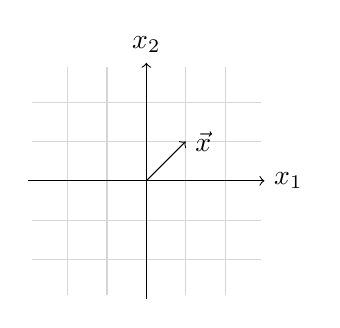
\begin{tikzpicture}[scale=0.5, ->]
        \draw[thin, color=black!20!white!80, -] (-2.9, -2.9) grid (2.9, 2.9);
        \draw (-3, 0) -- (3, 0) node[right] {$x_1$};
        \draw (0, -3) -- (0, 3) node[above] {$x_2$};

        \draw (0, 0) -- (1, 1) node [right] {$\vec{x}$};
    \end{tikzpicture}}
    \caption{Original Vector}
  \end{subfigure}
  \hfill
  \begin{subfigure}{0.32\linewidth}
    \resizebox{\linewidth}{!}{
      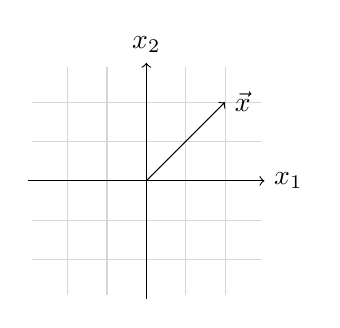
\begin{tikzpicture}[scale=0.5, ->]
        \draw[thin, color=black!20!white!80, -] (-2.9, -2.9) grid (2.9, 2.9);
        \draw (-3, 0) -- (3, 0) node[right] {$x_1$};
        \draw (0, -3) -- (0, 3) node[above] {$x_2$};

        \draw (0, 0) -- (2, 2) node [right] {$\vec{x}$};
    \end{tikzpicture}}
    \caption{Vector scaled by $c = 2$}
  \end{subfigure}
  \hfill
  \begin{subfigure}{0.32\linewidth}
    \resizebox{\linewidth}{!}{
      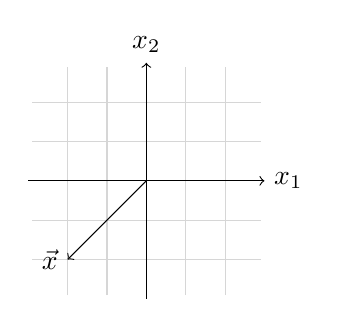
\begin{tikzpicture}[scale=0.5, ->]
        \draw[thin, color=black!20!white!80, -] (-2.9, -2.9) grid (2.9, 2.9);
        \draw (-3, 0) -- (3, 0) node[right] {$x_1$};
        \draw (0, -3) -- (0, 3) node[above] {$x_2$};

        \draw (0, 0) -- (-2, -2) node [left] {$\vec{x}$};
    \end{tikzpicture}}
    \caption{Vector scaled by $c = -2$}
  \end{subfigure}
  \caption{Vectors with constant multiplication applied}
  \label{fig:const_scale}
\end{figure}

\begin{defn}[Subtraction]
  Vector subtraction can be seen as reversing a vector before adding it. For instance if you are subtracting $\vec{x} - \vec{y}$, it's equivalent to $\vec{x} + (-\vec{y})$.

  Let $\vec{c} = \vec{a} - \vec{b}$. The result can be seen in Figure \ref{fig:vec_sub}.
\end{defn}
  \begin{figure}[h]
    \centering
    \begin{tikzpicture}[scale=2, ->]
      \draw[thin, color=black!20!white!80, -] (-2.9, -2.9) grid (2.9, 2.9);
      \draw (-3, 0) -- (3, 0) node[right] {$x_1$};
      \draw (0, -3) -- (0, 3) node[above] {$x_2$};

      \draw (0, 0) -- (1, 2.5) node[midway, anchor=south east] {$\vec{a}$};
      \draw (0, 0) -- (2, 1.5) node[midway, anchor=north] {$\vec{b}$};
      \draw[style=dashed, color=gray] (0, 0) -- (-2, -1.5) node[midway, anchor=north] {$\vec{b}$};
      \draw[style=dashed, color=gray] (1, 2.5) -- (-1, 1) node[midway, anchor=north west] {$\vec{b}$};
      \draw[color=red] (0, 0) -- (-1, 1) node[anchor=north east] {$\vec{c}$};
    \end{tikzpicture}
    \caption{Difference of two vectors in $\R^2$}
    \label{fig:vec_sub}
  \end{figure}

\subsection{Vectors between Points}
Let $A$ and $B$ represent points in space.
\begin{itemize}
\item A vector between $A$ and $B$ can be denoted as $\vec{AB}$
\item $A$ and $B$ can be treated as vectors from the origin $\vec{OA}$ and $\vec{OB}$
\item $\vec{AB}$ between $A$ and $B$ can be expressed as $\vec{OB} - \vec{OA}$
\item Less exlicitly, $\vec{A}$ and $\vec{B}$ are technically equivalent since the origin is implied as the source
\end{itemize}

\begin{exl}[Vector between points]
  Given $A = (1, 2)$ and $B = (2, 1)$, the vectors can be respresented as follows:
  \begin{equation*}
    \vec{OA} = \begin{bmatrix} 1\\2 \end{bmatrix},\quad
    \vec{OB} = \begin{bmatrix} 2\\1 \end{bmatrix}
  \end{equation*}
  Thus,
  \begin{equation*}
    \vec{AB} = \vec{OB} - \vec{OA} = \begin{bmatrix} 1\\2 \end{bmatrix} - \begin{bmatrix} 2\\1 \end{bmatrix} = \begin{bmatrix} -1\\1 \end{bmatrix}
  \end{equation*}

  This is graphically represented in Figure \ref{fig:vec_between_points}.
\end{exl}
\begin{figure}[h]
  \centering
  \begin{tikzpicture}[scale=2, ->]
    \draw[thin, color=black!20!white!80, -] (-0.9, -0.9) grid (2.9, 2.9);

    \draw (0, 0) -- (1, 2) node[midway, left] {$\vec{OA}$};
    \draw (0, 0) -- (2, 1) node[midway, right] {$\vec{OB}$};

    \draw[color=red] (1, 2) -- (2, 1) node[midway, above] {$\vec{AB}$};
    \draw (-1, 0) -- (3, 0) node[right] {$x_1$};
    \draw (0, -1) -- (0, 3) node[above] {$x_2$};

    \draw[fill=black] (1, 2) circle(0.05) node[left] {$A$};
    \draw[fill=black] (2, 1) circle(0.05) node[right] {$B$};
  \end{tikzpicture}
  \caption{Illustration of a vector between two points}
  \label{fig:vec_between_points}
\end{figure}

\subsection{Vector Magnitudes}
\begin{defn}[Vector Norm]

  Let $\vec{x} \in \R^n$
  The norm of x is defined as $\norm{vec{x}} = \sqrt{x_1^2 + x_2^2 + \cdots + x_{n-1}^2 + x_n^2}$, Derivec from the Pythagorean Theorem.
\end{defn}
\begin{itemize}
\item The norm of the standard basis vector is 1
\end{itemize}

\begin{defn}[Unit Vector]
\begin{equation*}
\norm{\vec{x}} = 1 \iff \vec{x} \text{ is unit vector}
\end{equation*}
\end{defn}
\begin{itemize}
\item All standard basis vectors are unit vectors
\item All vectors divided by norm are unit vectors
  \begin{itemize}
  \item Results in ``normalized vector,'' notated as $\hat{x}$
  \item $\hat{x} - \frac{\vec{x}}{\norm{\vec{x}}}$
  \end{itemize}
\end{itemize}

\begin{defn}[Distance Between Vectors]

  Given $\vec{x}$ and $\vec{y}$, the distance is $\norm{\vec{x} - \vec{y}}$
\end{defn}
\begin{itemize}
\item Allows us to analyze geometric quantities in $n$-dimensional space
  \begin{itemize}
  \item Important for analysis of space beyond 3 dimensions
  \end{itemize}
\item Reflects ``similarity'' of vectors
\end{itemize}

\begin{thm}[Properties of Norms]
  \begin{enumerate}
  \item\label{item:1} $\norm{\vec{x}} \geq 0,\quad \norm{\vec{x}} = 0 \iff \vec{x} = \vec{0}$
  \item\label{item:2} $\norm{c\vec{x}} = \abs{c} \cdot \norm{\vec{x}}$
    \item\label{item:3} $\norm{\vec{x} + \vec{y}} \leq \norm{\vec{x}} + \norm{\vec{y}}$
  \end{enumerate}
\end{thm}
\begin{itemize}
\item Item 3 is referred to as the triangle inequality
  \begin{itemize}
  \item For $\norm{\vec{x} + \vec{y} + \ldots}$, triangle inequality can be applied inductively
  \end{itemize}
\end{itemize}

\subsection{Angles}
\begin{defn}

  Let $\vec{x}, \vec{y} \in \R$
  
  The dot product of $\vec{x}$ and $\vec{y}$, $\vec{x} \cdot \vec{y}$, is given by
  \begin{equation*}
    \begin{bmatrix} x_1\\x_2\\\vdots\\x_{n-1}\\x_n\end{bmatrix} \cdot \begin{bmatrix}y_1\\y_2\\\vdots\\y_{n-1}\\y_n\end{bmatrix} = x_1y_1 + x_2y_2 + \ldots + x_{n-1}y_{n-1} + x_ny_n
  \end{equation*}
\end{defn}

\begin{thm}

  In $\R^2$, if $\vec{x}, \vec{y} \in \R^2$ and $\vec{x}, \vec{y} \neq \vec{0}$, let $\theta$ be the angle between those two vectors. Then:
  \begin{equation*}
    \vec{x} * \vec{y} = \norm{\vec{x}} \times \vec{y} \times \cos{\theta}
  \end{equation*}
\end{thm}
\begin{itemize}
\item Form of the cosine law
\end{itemize}

\end{document}
